\documentclass[conference]{IEEEtran}
\IEEEoverridecommandlockouts
% The preceding line is only needed to identify funding in the first footnote. If that is unneeded, please comment it out.

\usepackage{cite}
\usepackage{amsmath,amssymb,amsfonts}
\usepackage{algorithmic}
\usepackage[printonlyused]{acronym}
\usepackage{graphicx}
\usepackage{textcomp}
%\usepackage[backend=bibtex,style=IEEEtr]{biblatex}


\def\BibTeX{{\rm B\kern-.05em{\sc i\kern-.025em b}\kern-.08em
    T\kern-.1667em\lower.7ex\hbox{E}\kern-.125emX}}
\begin{document}

\title{Activity Recognition with mobile devices\\
}

\author{\IEEEauthorblockN{1\textsuperscript{st} Simon Angerbauer}
\IEEEauthorblockA{\textit{Mobile Computing} \\
\textit{University Of Applied Sciences Upper Austria}\\
Hagenberg, Austria \\
simon.angerbauer@students.fh-hagenberg.at}
\and
\IEEEauthorblockN{2\textsuperscript{nd} Paul Schmutz}
\IEEEauthorblockA{\textit{Mobile Computing} \\
\textit{University Of Applied Sciences Upper Austria}\\
Hagenberg, Austria \\
paul.schmutz@students.fh-hagenberg.at}
\and
\IEEEauthorblockN{3\textsuperscript{rd} Roman Socovka}
\IEEEauthorblockA{\textit{Mobile Computing} \\
\textit{University Of Applied Sciences Upper Austria}\\
Hagenberg, Austria \\
roman.socovka@students.fh-hagenberg.at}
}

\maketitle

\begin{abstract}
This document is a model and instructions for \LaTeX.
This and the IEEEtran.cls file define the components of your paper [title, text, heads, etc.]. *CRITICAL: Do Not Use Symbols, Special Characters, Footnotes, 
or Math in Paper Title or Abstract.
\\
\\
\\
\\
\\
\\
\\
\\
\\
\\
\\
\\
\\
\\
\\
\\
TODO
\end{abstract}

\begin{IEEEkeywords}
Human Activity Recognition, accelerometer, movement pattern detection
\end{IEEEkeywords}

\section{Introduction -- Simon}
asdfas
\\
\\
\\
\\
\\
\\
\\
\\
\\
\\
\\
\\
\\
\\
\\
\\
\\
\\
\\
\\
\\
\\
\\
\\
\\
\\
\\
\\
\\
\\
\\
\\
\\
\\
\\
\\
\\
\\
\\
\\
\\
\\
\\
\\
\\
\\
\\
\\
\\
\\
\\
\\
\\
\\
\\
\\
intro


\section{Related Work -- Paul}
As activity recognition - especially \ac{HAR} - is a popular topic, there already many studies and papers recording detection of gestures in both natural and laboratory settings as well as using regular mobile accelerometers and multiple high-performant accelerometers attached to different parts of the body.

Although the use of multiple separate acceleration sensor devices can improve results drastically up to 80\% and more ~\cite{Bao2004}, cell phones are the easiest solution to spread the capability of measuring and classifying movement patterns.
\begin{figure}[!htb]
\centering
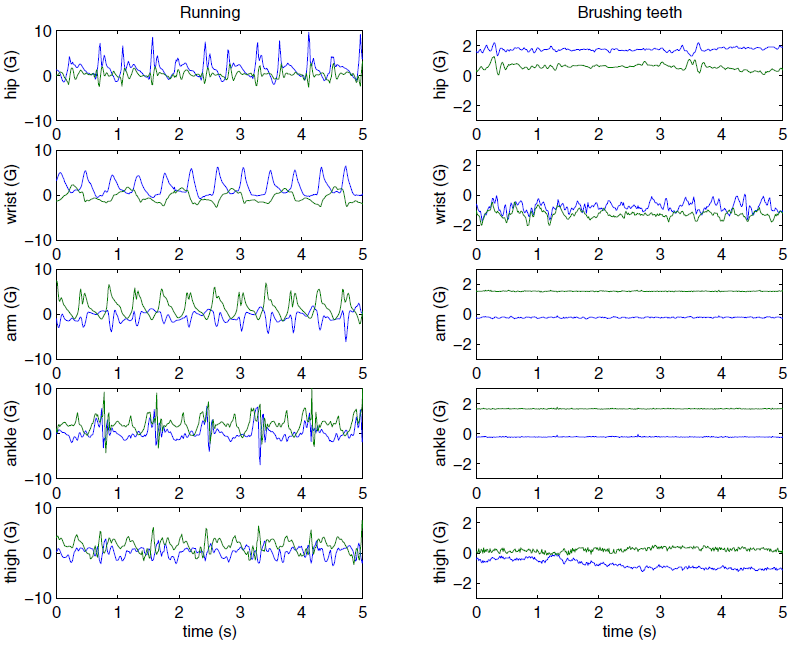
\includegraphics[width=\linewidth]{multiple_accelerometers}
\caption{As noted by Bao and Intille ~\cite{Bao2004} this picture shows the use of five accelerometers placed on the described body parts. Multiple accelerometers allow more accurate detection but is also complex and only suitable in laboratory conditions when compared to mobile device accelerometers.}
\label{fig:multipleAccelerometers}
\end{figure}
The use of smartphone sensors is not only practicable but also allows developing applications at low-cost ~\cite{Brezmes2009}.

Cell phones however are disadvantageous to the effect that the device tilt is uncertain oftentimes ~\cite{Brezmes2009}. So sensor data for a particular movement patterns may differ from each other significantly. Under that circumstance algorithms therefore are far more complex and their results more inaccurate. In one approach for instance the orientation of the tri-axial sensor is used to distinguish between standing and sitting ~\cite{Kwapisz2011}, which is not a real-world scenario for everybody as every individual user might carry the phone in a different way. As the performance of algorithms and devices have increased, the problems of phone orientation can be dealt with by now. Also wearing the sensor at different body parts is worsening the situation. Therefore a training phase combined with an \ac{AI} learning algorithm can help to improve detection results ~\cite{Kwapisz2011,Bao2004}. Most studies discussing activity recognition with mobile devices usually introduce training phases for collecting sensor data. For example each individual user has a preferred way to hold the phone, like a chest pocket, front trousers pocket, a rear trousers pocket, an inner jacket pocket, \dots ~\cite{Brezmes2009}. This is essential as different sensor placement on the body produce different acceleration data. The experimental results show that when the sensor is placed on different rigid body, different models are required for certain activities ~\cite{Henpraserttae2011}.

While multi-sensor approaches focus on detecting a large set of activities ~\cite{Bao2004}, many studies that make use of just one triaxial smartphone accelerometer are concentrating on a smaller subset like walking, jogging, ascending stairs, descending stairs, sitting and standing which is sufficient for detecting standard activities of most people's everyday lives.

A critical point is real-time detection of gestures. Analyzing data beforehand is necessary in order to recognize certain movement patterns. Real-time capability of systems can be essential for detecting running in a sports and health application or even monitoring aged people or anyone under medical control ~\cite{Brezmes2009}. Today's mobile devices have enough computing power to collect and detect for example a fall which as a emergency requires fast reaction. The solution of handling calculations on the mobile device is also highly scalable as no additional server is necessary for data processing ~\cite{Kwapisz2011}.

As mobile devices nowadays are highly connective and come with additional sensors such as \ac{GPS} sensors, vision sensors, audio sensors, light sensors, temperature sensors or direction sensors ~\cite{Kwapisz2011}, activity recognition offers even more possibilities. The availability of these technologies creates new data mining opportunities ~\cite{Kwapisz2011}.

Energy saving on mobile devices by using different sampling frequencies, for example \ac{GPS} need a lot of power as well sensors \dots
\\
\\
\\
\\
\\
\\
\\
\\
\\
\\
\\
\\
\\
\\
\\
\subsection{Subsection blabla}
subsection
\newpage
\section{Evaluation -- Simon}

\subsection{Results}
\begin{figure}[!htb]
  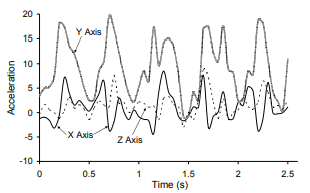
\includegraphics[width=\linewidth]{walking.png}
  \caption{Walking}
  \label{fig:walking}
\end{figure}
\begin{figure}[!htb]
  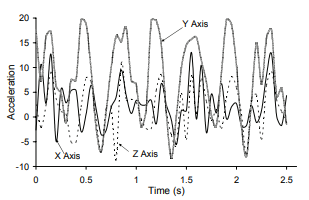
\includegraphics[width=\linewidth]{jogging.png}
  \caption{Jogging}
  \label{fig:jogging}
\end{figure}
\begin{figure}[!htb]
  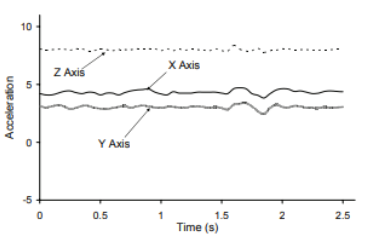
\includegraphics[width=\linewidth]{sitting.png}
  \caption{Sitting}
  \label{fig:sitting}
\end{figure}
\begin{figure}[!htb]
  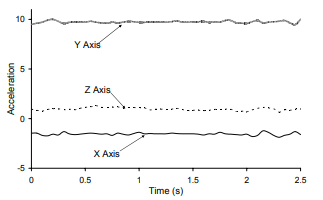
\includegraphics[width=\linewidth]{standing.png}
  \caption{Standing}
  \label{fig:standing}
\end{figure}
\begin{figure}[!htb]
  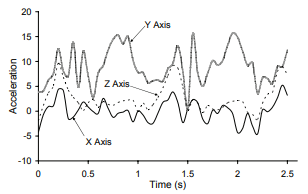
\includegraphics[width=\linewidth]{ascending_stairs.png}
  \caption{Ascending Stairs}
  \label{fig:ascendingStairs}
\end{figure}
\begin{figure}[!htb]
  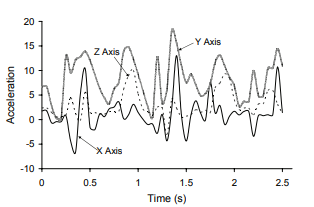
\includegraphics[width=\linewidth]{descending_stairs.png}
  \caption{Descending Stairs}
  \label{fig:descendingStairs}
\end{figure}

\newpage
\subsection{Analysis}

TODO some analysis shit

\section{Conclusion -- Paul}
The use of smartphones for activity recognition is appropriate to achieve a high number of users, however it not the most accurate approach.
Smart wearable devices are getting more popular, which could allow the use of multiple sensors increasing accuracy of gesture detection. As there is a large variety of such wearables and the majority still owns one single cell smartphone, attaching multiple accelerometers  on different parts of the body generally is not a natural use-case. We think that focusing on a high number of users by concentrating on evaluating just smartphone sensor data is significant, as the goal is to give as many people as possible access to the technology of activity recognition.
Cell phone accelerometer data still can be enhanced by developing more sophisticated software processing sensor data and learning user behaviors, so that a basic set of gestures like walking, standing or climbing stairs can be detected maintaining a low error rate while keeping the number of users at an upper level.
Although activity data is sensitive information for each individual user, it is valuable for statistical researches. By obtaining movement patterns of a high number of users many different insights of the world's population can be won. This would also contribute in improving a persons lifestyle, for example by helping him find an appropriate amount of exercise. As smartphones are highly connected to the internet this process can be automatized and reported to the user in real-time. Also comparing activity data between users might increase the willingness of people doing sports and prevent medical risks.

Could be important for the health, aging, monitoring people under medical control

\section*{List of Abbreviations}
\begin{acronym}[XXXXXXXX]
 \acro{AI}{Artificial Intelligence}
 \acro{GPS}{Global Positioning System}
 \acro{HAR}{Human Activity Recognition} 
\end{acronym}

\addcontentsline{toc}{section}{References}
\bibliographystyle{unsrt}
\bibliography{references}
%%%----------------------------------------------------------
%\MakeBibliography                        				% references
%%%----------------------------------------------------------
%\printbibliography
%\bibliography{references}  	% name of bibliography file (references.bib)
%\bibliographystyle{ieeetr}
\end{document}
